\panel{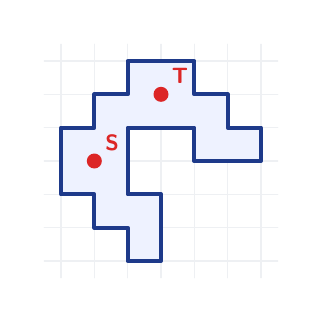
\begin{tikzpicture}[x=1bp, y=1bp]\path[use as bounding box] (0,0) rectangle (96.00,96.00);\clip (0,0) rectangle (96.00,96.00);
\path[draw={rgb,255:red,238;green,240;blue,243}, line width=0.52bp, line cap=round, line join=round] (12.00,6.00) -- (12.00,90.00);
\path[draw={rgb,255:red,238;green,240;blue,243}, line width=0.52bp, line cap=round, line join=round] (24.00,6.00) -- (24.00,90.00);
\path[draw={rgb,255:red,238;green,240;blue,243}, line width=0.52bp, line cap=round, line join=round] (36.00,6.00) -- (36.00,90.00);
\path[draw={rgb,255:red,238;green,240;blue,243}, line width=0.52bp, line cap=round, line join=round] (48.00,6.00) -- (48.00,90.00);
\path[draw={rgb,255:red,238;green,240;blue,243}, line width=0.52bp, line cap=round, line join=round] (60.00,6.00) -- (60.00,90.00);
\path[draw={rgb,255:red,238;green,240;blue,243}, line width=0.52bp, line cap=round, line join=round] (72.00,6.00) -- (72.00,90.00);
\path[draw={rgb,255:red,238;green,240;blue,243}, line width=0.52bp, line cap=round, line join=round] (84.00,6.00) -- (84.00,90.00);
\path[draw={rgb,255:red,238;green,240;blue,243}, line width=0.52bp, line cap=round, line join=round] (6.00,12.00) -- (90.00,12.00);
\path[draw={rgb,255:red,238;green,240;blue,243}, line width=0.52bp, line cap=round, line join=round] (6.00,24.00) -- (90.00,24.00);
\path[draw={rgb,255:red,238;green,240;blue,243}, line width=0.52bp, line cap=round, line join=round] (6.00,36.00) -- (90.00,36.00);
\path[draw={rgb,255:red,238;green,240;blue,243}, line width=0.52bp, line cap=round, line join=round] (6.00,48.00) -- (90.00,48.00);
\path[draw={rgb,255:red,238;green,240;blue,243}, line width=0.52bp, line cap=round, line join=round] (6.00,60.00) -- (90.00,60.00);
\path[draw={rgb,255:red,238;green,240;blue,243}, line width=0.52bp, line cap=round, line join=round] (6.00,72.00) -- (90.00,72.00);
\path[draw={rgb,255:red,238;green,240;blue,243}, line width=0.52bp, line cap=round, line join=round] (6.00,84.00) -- (90.00,84.00);
\path[draw={rgb,255:red,30;green,58;blue,138}, line width=1.50bp, fill={rgb,255:red,238;green,242;blue,255}, line join=round] (12.00,36.00) -- (12.00,60.00) -- (24.00,60.00) -- (24.00,72.00) -- (36.00,72.00) -- (36.00,84.00) -- (60.00,84.00) -- (60.00,72.00) -- (72.00,72.00) -- (72.00,60.00) -- (84.00,60.00) -- (84.00,48.00) -- (60.00,48.00) -- (60.00,60.00) -- (36.00,60.00) -- (36.00,36.00) -- (48.00,36.00) -- (48.00,12.00) -- (36.00,12.00) -- (36.00,24.00) -- (24.00,24.00) -- (24.00,36.00) -- cycle;
\path[fill={rgb,255:red,220;green,38;blue,38}] (24.00,48.00) circle[radius=2.70bp];
\node[anchor=base west, text={rgb,255:red,220;green,38;blue,38}, font=\fontsize{8.2}{9.9}\selectfont\sffamily\bfseries, inner sep=0pt] at (27.75,51.75) {S};
\path[fill={rgb,255:red,220;green,38;blue,38}] (48.00,72.00) circle[radius=2.70bp];
\node[anchor=base west, text={rgb,255:red,220;green,38;blue,38}, font=\fontsize{8.2}{9.9}\selectfont\sffamily\bfseries, inner sep=0pt] at (51.75,75.75) {T};
\end{tikzpicture}}{(a) straight}\hspace{16.5bp}\panel{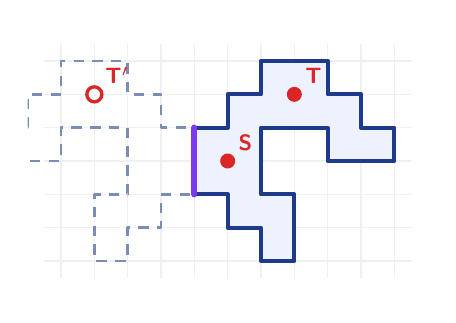
\begin{tikzpicture}[x=1bp, y=1bp]\path[use as bounding box] (0,0) rectangle (144.00,96.00);\clip (0,0) rectangle (144.00,96.00);
\path[draw={rgb,255:red,238;green,240;blue,243}, line width=0.52bp, line cap=round, line join=round] (12.00,6.00) -- (12.00,90.00);
\path[draw={rgb,255:red,238;green,240;blue,243}, line width=0.52bp, line cap=round, line join=round] (24.00,6.00) -- (24.00,90.00);
\path[draw={rgb,255:red,238;green,240;blue,243}, line width=0.52bp, line cap=round, line join=round] (36.00,6.00) -- (36.00,90.00);
\path[draw={rgb,255:red,238;green,240;blue,243}, line width=0.52bp, line cap=round, line join=round] (48.00,6.00) -- (48.00,90.00);
\path[draw={rgb,255:red,238;green,240;blue,243}, line width=0.52bp, line cap=round, line join=round] (60.00,6.00) -- (60.00,90.00);
\path[draw={rgb,255:red,238;green,240;blue,243}, line width=0.52bp, line cap=round, line join=round] (72.00,6.00) -- (72.00,90.00);
\path[draw={rgb,255:red,238;green,240;blue,243}, line width=0.52bp, line cap=round, line join=round] (84.00,6.00) -- (84.00,90.00);
\path[draw={rgb,255:red,238;green,240;blue,243}, line width=0.52bp, line cap=round, line join=round] (96.00,6.00) -- (96.00,90.00);
\path[draw={rgb,255:red,238;green,240;blue,243}, line width=0.52bp, line cap=round, line join=round] (108.00,6.00) -- (108.00,90.00);
\path[draw={rgb,255:red,238;green,240;blue,243}, line width=0.52bp, line cap=round, line join=round] (120.00,6.00) -- (120.00,90.00);
\path[draw={rgb,255:red,238;green,240;blue,243}, line width=0.52bp, line cap=round, line join=round] (132.00,6.00) -- (132.00,90.00);
\path[draw={rgb,255:red,238;green,240;blue,243}, line width=0.52bp, line cap=round, line join=round] (6.00,12.00) -- (138.00,12.00);
\path[draw={rgb,255:red,238;green,240;blue,243}, line width=0.52bp, line cap=round, line join=round] (6.00,24.00) -- (138.00,24.00);
\path[draw={rgb,255:red,238;green,240;blue,243}, line width=0.52bp, line cap=round, line join=round] (6.00,36.00) -- (138.00,36.00);
\path[draw={rgb,255:red,238;green,240;blue,243}, line width=0.52bp, line cap=round, line join=round] (6.00,48.00) -- (138.00,48.00);
\path[draw={rgb,255:red,238;green,240;blue,243}, line width=0.52bp, line cap=round, line join=round] (6.00,60.00) -- (138.00,60.00);
\path[draw={rgb,255:red,238;green,240;blue,243}, line width=0.52bp, line cap=round, line join=round] (6.00,72.00) -- (138.00,72.00);
\path[draw={rgb,255:red,238;green,240;blue,243}, line width=0.52bp, line cap=round, line join=round] (6.00,84.00) -- (138.00,84.00);
\path[draw={rgb,255:red,124;green,141;blue,181}, line width=1.05bp, dash pattern=on 3.75bp off 3.00bp, line join=round] (60.00,36.00) -- (60.00,60.00) -- (48.00,60.00) -- (48.00,72.00) -- (36.00,72.00) -- (36.00,84.00) -- (12.00,84.00) -- (12.00,72.00) -- (0.00,72.00) -- (0.00,60.00) -- (-12.00,60.00) -- (-12.00,48.00) -- (12.00,48.00) -- (12.00,60.00) -- (36.00,60.00) -- (36.00,36.00) -- (24.00,36.00) -- (24.00,12.00) -- (36.00,12.00) -- (36.00,24.00) -- (48.00,24.00) -- (48.00,36.00) -- cycle;
\path[draw={rgb,255:red,30;green,58;blue,138}, line width=1.50bp, fill={rgb,255:red,238;green,242;blue,255}, line join=round] (60.00,36.00) -- (60.00,60.00) -- (72.00,60.00) -- (72.00,72.00) -- (84.00,72.00) -- (84.00,84.00) -- (108.00,84.00) -- (108.00,72.00) -- (120.00,72.00) -- (120.00,60.00) -- (132.00,60.00) -- (132.00,48.00) -- (108.00,48.00) -- (108.00,60.00) -- (84.00,60.00) -- (84.00,36.00) -- (96.00,36.00) -- (96.00,12.00) -- (84.00,12.00) -- (84.00,24.00) -- (72.00,24.00) -- (72.00,36.00) -- cycle;
\path[draw={rgb,255:red,124;green,58;blue,237}, line width=2.25bp, line cap=round, line join=round] (60.00,36.00) -- (60.00,60.00);
\path[fill={rgb,255:red,220;green,38;blue,38}] (72.00,48.00) circle[radius=2.70bp];
\node[anchor=base west, text={rgb,255:red,220;green,38;blue,38}, font=\fontsize{8.2}{9.9}\selectfont\sffamily\bfseries, inner sep=0pt] at (75.75,51.75) {S};
\path[fill={rgb,255:red,220;green,38;blue,38}] (96.00,72.00) circle[radius=2.70bp];
\node[anchor=base west, text={rgb,255:red,220;green,38;blue,38}, font=\fontsize{8.2}{9.9}\selectfont\sffamily\bfseries, inner sep=0pt] at (99.75,75.75) {T};
\path[draw={rgb,255:red,220;green,38;blue,38}, line width=1.20bp, fill=white] (24.00,72.00) circle[radius=2.70bp];
\node[anchor=base west, text={rgb,255:red,220;green,38;blue,38}, font=\fontsize{8.2}{9.9}\selectfont\sffamily\bfseries, inner sep=0pt] at (27.75,75.75) {T$'$};
\end{tikzpicture}}{(b) mirror across $x = -1$}\hspace{16.5bp}\panel{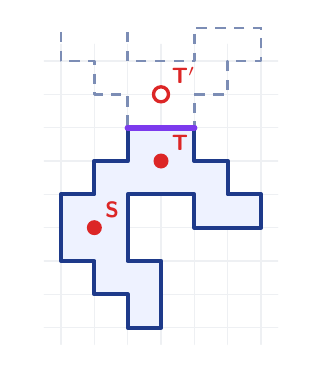
\begin{tikzpicture}[x=1bp, y=1bp]\path[use as bounding box] (0,0) rectangle (96.00,120.00);\clip (0,0) rectangle (96.00,120.00);
\path[draw={rgb,255:red,238;green,240;blue,243}, line width=0.52bp, line cap=round, line join=round] (12.00,6.00) -- (12.00,114.00);
\path[draw={rgb,255:red,238;green,240;blue,243}, line width=0.52bp, line cap=round, line join=round] (24.00,6.00) -- (24.00,114.00);
\path[draw={rgb,255:red,238;green,240;blue,243}, line width=0.52bp, line cap=round, line join=round] (36.00,6.00) -- (36.00,114.00);
\path[draw={rgb,255:red,238;green,240;blue,243}, line width=0.52bp, line cap=round, line join=round] (48.00,6.00) -- (48.00,114.00);
\path[draw={rgb,255:red,238;green,240;blue,243}, line width=0.52bp, line cap=round, line join=round] (60.00,6.00) -- (60.00,114.00);
\path[draw={rgb,255:red,238;green,240;blue,243}, line width=0.52bp, line cap=round, line join=round] (72.00,6.00) -- (72.00,114.00);
\path[draw={rgb,255:red,238;green,240;blue,243}, line width=0.52bp, line cap=round, line join=round] (84.00,6.00) -- (84.00,114.00);
\path[draw={rgb,255:red,238;green,240;blue,243}, line width=0.52bp, line cap=round, line join=round] (6.00,12.00) -- (90.00,12.00);
\path[draw={rgb,255:red,238;green,240;blue,243}, line width=0.52bp, line cap=round, line join=round] (6.00,24.00) -- (90.00,24.00);
\path[draw={rgb,255:red,238;green,240;blue,243}, line width=0.52bp, line cap=round, line join=round] (6.00,36.00) -- (90.00,36.00);
\path[draw={rgb,255:red,238;green,240;blue,243}, line width=0.52bp, line cap=round, line join=round] (6.00,48.00) -- (90.00,48.00);
\path[draw={rgb,255:red,238;green,240;blue,243}, line width=0.52bp, line cap=round, line join=round] (6.00,60.00) -- (90.00,60.00);
\path[draw={rgb,255:red,238;green,240;blue,243}, line width=0.52bp, line cap=round, line join=round] (6.00,72.00) -- (90.00,72.00);
\path[draw={rgb,255:red,238;green,240;blue,243}, line width=0.52bp, line cap=round, line join=round] (6.00,84.00) -- (90.00,84.00);
\path[draw={rgb,255:red,238;green,240;blue,243}, line width=0.52bp, line cap=round, line join=round] (6.00,96.00) -- (90.00,96.00);
\path[draw={rgb,255:red,238;green,240;blue,243}, line width=0.52bp, line cap=round, line join=round] (6.00,108.00) -- (90.00,108.00);
\path[draw={rgb,255:red,124;green,141;blue,181}, line width=1.05bp, dash pattern=on 3.75bp off 3.00bp, line join=round] (12.00,132.00) -- (12.00,108.00) -- (24.00,108.00) -- (24.00,96.00) -- (36.00,96.00) -- (36.00,84.00) -- (60.00,84.00) -- (60.00,96.00) -- (72.00,96.00) -- (72.00,108.00) -- (84.00,108.00) -- (84.00,120.00) -- (60.00,120.00) -- (60.00,108.00) -- (36.00,108.00) -- (36.00,132.00) -- (48.00,132.00) -- (48.00,156.00) -- (36.00,156.00) -- (36.00,144.00) -- (24.00,144.00) -- (24.00,132.00) -- cycle;
\path[draw={rgb,255:red,30;green,58;blue,138}, line width=1.50bp, fill={rgb,255:red,238;green,242;blue,255}, line join=round] (12.00,36.00) -- (12.00,60.00) -- (24.00,60.00) -- (24.00,72.00) -- (36.00,72.00) -- (36.00,84.00) -- (60.00,84.00) -- (60.00,72.00) -- (72.00,72.00) -- (72.00,60.00) -- (84.00,60.00) -- (84.00,48.00) -- (60.00,48.00) -- (60.00,60.00) -- (36.00,60.00) -- (36.00,36.00) -- (48.00,36.00) -- (48.00,12.00) -- (36.00,12.00) -- (36.00,24.00) -- (24.00,24.00) -- (24.00,36.00) -- cycle;
\path[draw={rgb,255:red,124;green,58;blue,237}, line width=2.25bp, line cap=round, line join=round] (36.00,84.00) -- (60.00,84.00);
\path[fill={rgb,255:red,220;green,38;blue,38}] (24.00,48.00) circle[radius=2.70bp];
\node[anchor=base west, text={rgb,255:red,220;green,38;blue,38}, font=\fontsize{8.2}{9.9}\selectfont\sffamily\bfseries, inner sep=0pt] at (27.75,51.75) {S};
\path[fill={rgb,255:red,220;green,38;blue,38}] (48.00,72.00) circle[radius=2.70bp];
\node[anchor=base west, text={rgb,255:red,220;green,38;blue,38}, font=\fontsize{8.2}{9.9}\selectfont\sffamily\bfseries, inner sep=0pt] at (51.75,75.75) {T};
\path[draw={rgb,255:red,220;green,38;blue,38}, line width=1.20bp, fill=white] (48.00,96.00) circle[radius=2.70bp];
\node[anchor=base west, text={rgb,255:red,220;green,38;blue,38}, font=\fontsize{8.2}{9.9}\selectfont\sffamily\bfseries, inner sep=0pt] at (51.75,99.75) {T$'$};
\end{tikzpicture}}{(c) mirror across $y = 3$}
